%%%%%%%%%%%%%%%%%%%%%%% file template.tex %%%%%%%%%%%%%%%%%%%%%%%%%
%
% This is a general template file for the LaTeX package SVJour3
% for Springer journals.          Springer Heidelberg 2010/09/16
%
% Copy it to a new file with a new name and use it as the basis
% for your article. Delete % signs as needed.
%
% This template includes a few options for different layouts and
% content for various journals. Please consult a previous issue of
% your journal as needed.
%
%%%%%%%%%%%%%%%%%%%%%%%%%%%%%%%%%%%%%%%%%%%%%%%%%%%%%%%%%%%%%%%%%%%
%
% First comes an example EPS file -- just ignore it and
% proceed on the \documentclass line
% your LaTeX will extract the file if required
\begin{filecontents*}{example.eps}
%!PS-Adobe-3.0 EPSF-3.0
%%BoundingBox: 19 19 221 221
%%CreationDate: Mon Sep 29 1997
%%Creator: programmed by hand (JK)
%%EndComments
gsave
newpath
  20 20 moveto
  20 220 lineto
  220 220 lineto
  220 20 lineto
closepath
2 setlinewidth
gsave
  .4 setgray fill
grestore
stroke
grestore
\end{filecontents*}
%
\RequirePackage{fix-cm}
%
%\documentclass{svjour3}                     % onecolumn (standard format)
%\documentclass[smallcondensed]{svjour3}     % onecolumn (ditto)
\documentclass[smallextended]{svjour3}       % onecolumn (second format)
%\documentclass[twocolumn]{svjour3}          % twocolumn
%
\smartqed  % flush right qed marks, e.g. at end of proof
%
\usepackage{graphicx}



\usepackage{rotate}
\usepackage{colortbl}
\usepackage{arydshln}
\usepackage{times}
\usepackage[dvipsnames]{xcolor}
\usepackage{rotating}
\usepackage{makecell} 
\usepackage{tabularx}
\usepackage{balance}
\usepackage{booktabs}
\usepackage{wrapfig}
\usepackage{tikz}
\usetikzlibrary{angles}
\usepackage{makecell}
\usepackage{tabu}
\usepackage{multirow}
\newcommand{\bi}{\begin{itemize}}
\newcommand{\ei}{\end{itemize}}
\newcommand{\be}{\begin{enumerate}}
\newcommand{\ee}{\end{enumerate}}
\newcommand{\fig}[1]{Figure~\ref{fig:#1}}
\newcommand{\eq}[1]{Equation~\ref{eq:#1}}
\newcommand{\tion}[1]{\S\ref{sect:#1}}



\usepackage{url}
%%% graph

\newcommand{\crule}[3][darkgray]{\textcolor{#1}{\rule{#2}{#3}}}

\newcommand{\dbox}[1] { \crule[black!#1]{0.67cm}{0.4cm} 
\hspace{-0.51cm}\scalebox{1}[1.0]{{\textcolor{black}{{\bf $^{#1}$}}}\hspace{0.1mm}}}


\newcommand{\wbox}[1] { \crule[black!#1]{0.67cm}{0.4cm} 
\hspace{-0.51cm}\scalebox{1}[1.0]{{\textcolor{white}{{\bf $^{#1}$}}}\hspace{0.1mm}}}


\newcommand{\quart}[4]{
\begin{picture}(100,6)%1
    {
        \color{black}
        \put(#3,3)
        {\circle*{4}}
        \put(#1,3)
        {\line(1,0){#2}}
    }
\end{picture}
}

\newcommand{\ofr} {
{\textit{out-of-range}}
}


\usepackage[framemethod=tikz]{mdframed}
\usetikzlibrary{shadows}
\usepackage{graphics}
\newmdenv[
tikzsetting= {fill=gray!10},
linewidth=1pt,
roundcorner=2pt, 
shadow=false
]{myshadowbox}

\newenvironment{result}[2]
{\begin{myshadowbox}\textbf{\textit{\underline{Lesson#1:}}} #2}{ 
\end{myshadowbox}}
    
\newcommand{\nm}[1]{\hline\multicolumn{1}{c}{\cellcolor{black} { {\bf \textcolor{white}{#1}}}}}
%\pdfoutput=1
%
% \usepackage{mathptmx}      % use Times fonts if available on your TeX system
%
% insert here the call for the packages your document requires
%\usepackage{latexsym}
% etc.
%
% please place your own definitions here and don't use \def but
% \newcommand{}{}
%
% Insert the name of "your journal" with
% \journalname{myjournal}
%
\begin{document}

\title{Hyperparameter Optimization  for    Effort Estimation
}
% \subtitle{Do you have a subtitle?\\ If so, write it here}

%\titlerunning{Short form of title}        % if too long for running head

\author{Tianpei Xia         \and
        Rahul Krishna         \and
        Jianfeng Chen         \and
        George Mathew         \and
        Xipeng Shen         \and
        Tim Menzies         
}

%\authorrunning{Short form of author list} % if too long for running head

\institute{Tianpei Xia \at
              Department of Computer Science, North Carolina State University, Raleigh, NC, USA \\
              \email{txia4@ncsu.edu}           %  \\
%             \emph{Present address:} of F. Author  %  if needed
           \and
           Tim Menzies \at
              Department of Computer Science, North Carolina State University, Raleigh, NC, USA \\
              \email{timm@ieee.org}
}

\date{the date of receipt and acceptance should be inserted later}
% The correct dates will be entered by the editor


\maketitle

\begin{abstract}
Software analytics has  been widely used in software engineering for many tasks such as 
generating effort estimates for  software projects. One of the ``black arts'' of software analytics is tuning the 
parameters controlling a  data mining algorithm.
Such {\em hyperparameter optimization} has been widely studied in other software analytics domains
(e.g. defect prediction and text mining) but, so far, has not been extensively explored for effort
estimation.
Accordingly, this paper seeks simple, automatic,     effective and fast methods
for finding good  tunings for  automatic software effort estimation.

We introduce a     hyperparameter optimization architecture called
  OIL  (Optimized Inductive Learning). 
  We test OIL  on a wide range of  hyperparameter optimizers using  
  data from 945 software projects. After tuning,
  large improvements in effort estimation accuracy were observed
  (measured in terms of the magnitude of the relative error and standardized accuracy).
  
  From those results, we recommend
  using  regression trees (CART) tuned by either different evolution or  MOEA/D.
This   particular combination of learner and optimizers often achieves
in one or two hours what other optimizers need days to weeks
of CPU time to accomplish.
 
   
An important part of this analysis is its reproducibility and refutability. All our scripts
and data are on-line. It is hoped that this paper will prompt and enable much more research on better methods
to tune software effort estimators.
\keywords{Effort Estimation \and Optimization \and Evolutionary algorithms}
% \PACS{PACS code1 \and PACS code2 \and more}
% \subclass{MSC code1 \and MSC code2 \and more}
\end{abstract}

\section{Introduction}
\label{intro}
This paper explores methods to improve algorithms
for software effort estimation.
This is needed since software  effort estimates   can be 
wildly inaccurate\cite{kemerer1987empirical}. Inadequate or overfull funding can cause a considerable waste of resource and time. For example, NASA canceled its  Check-out Launch Control System project after the initial \$200M estimate was exceeded by another \$200M~\cite{cowing02}. Effort estimations need to be accurate  (if for
no other reason) since many government
organizations demand that the budgets allocated to
large publicly funded projects be double-checked by some estimation model~\cite{MenziesNeg:2017}.  
Non-algorithm techniques that rely on human judgment~\cite{jorgensen2004review} are much harder to  
audit or 
dispute (e.g.,  when the estimate is generated by a senior colleague but disputed by others). 

Sarro et al.~\cite{sarro2016multi} assert that effort  estimation  is  a  critical  activity  for  planning  and
monitoring software project development in order to deliver
the  product  on  time  and  within  budget~\cite{briand2002resource,kocaguneli2011experiences,trendowicz2014software}.   The
competitiveness (and occasionally the survival) of software
organizations depends on their ability to accurately predict
the  effort  required  for  developing  software  systems;  both
over- or under- estimates can negatively affect the outcome
of software projects~\cite{trendowicz2014software,mcconnell2006software,mendes2002further,sommerville2010software}.



{\em Hyperparameter optimization}  is the automatic tuning
of the control parameters of a data
mining algorithm.
It is well established that  classification tasks like software defect prediction or 
 text classification are improved by such tuning~\cite{Fu2016TuningFS,tanti18,AGRAWAL2018,agrawal2017better}.
But as discussed below (see  \S\ref{sec:4}), the  benefits of     hyperparameter optimization for   effort estimation 
have not been extensively
studied.  Accordingly, this paper investigates hyperparameter optimization using data from 945   projects.
To the best of our knowledge,
this study is the most extensive exploration  of
hyperparameter optimization and effort estimation yet undertaken. 

We assess our results with respect to recent comments by 
Acuri \& Fraser~\cite{Arcuri2013}.
They caution that to transition hyperparameter optimizers  to industry,   they need to be {\bf  fast}:
\begin{quote}
{\em  
A practitioner, that wants to use such tools, should not be required to run large tuning phases before being able to apply those tools~\cite{Arcuri2013}.}
\end{quote}
Also,  according to Acuri \& Fraser, optimizers must  be {\bf useful}:
\begin{quote}
{\em At least in the context of test data generation, (tuning) does not seem easy to find good settings that significantly outperform   ``default'' values. ... Using ``default'' values is a reasonable and justified choice, whereas parameter tuning is a long and expensive process that might or might not pay off~\cite{Arcuri2013}.}
\end{quote}
Hence, to  check the value of hyperparamter optimization for effort estimation, we ask the following research questions.


{\bf RQ1:} To address one concern raised by Acuri \& Fraser,
 we must  first ask {\em is it best   to just  use ``off-the-shelf'' defaults?}
We will find that  tuned learners
provide  better estimates  than untuned learners. Hence, for effort estimation:
 \begin{result}{1}
 ``off-the-shelf'' defaults should be deprecated.
 \end{result}

{\bf RQ2:} An alternate form of the first question is to ask if all this tuning
 effort can be avoided if   we {\em  replace the old defaults with new defaults}
 This  checks is we can run tuning once (and once only) then use those new defaults
 ever after. It will be seen that effort estimation tunings differ, quite dramatically,
 from data set to data set. Hence, for effort estimation:
 \begin{result}{2}
 Overall, there are no ``best'' default settings.
 \end{result}

{\bf RQ3:}  The first two research questions tell us that we must retune
our effort estimators whenever new data arrives. Accordingly, we must now address the other concern raised by Acuri \& Fraser
about CPU cost. Hence, in this question we ask   {\em can we avoid  
slow hyperparameter optimization}? The answer to  {\bf RQ3} will be ``yes'' since
our results show that for effort estimation:
 \begin{result}{3}
 Overall, our slowest optimizers  perform no better than certain faster ones.
 \end{result}


{\bf RQ4:} The
final question to  answer is {\em what  hyperparameter   optimizers  to  use  for  effort
estimation?} Here, we report that a certain combination  of learners and optimizers usually
produce best results. Further, this
particular combination  often achieves in one or two
hours what other optimizers need days to weeks of CPU to achieve. Hence we will recommend 
the following combination for effort estimation:
\begin{result}{4}
For new data sets, try {\em CART} with the optimizers  {\em MOEA/D} or 
{\em differential evolution}.
\end{result}
(Note: The {\it italicized} words are explained below.)

In summary, unlike the test case generation domains explored by Acuri \& Fraser,
hyperparamter optimization for effort estimation is both {\bf useful} and {\bf fast}.


Overall the contributions of this paper are:
\bi
\item A demonstration that defaults settings are not the best way to perform effort estimation. Hence, when new
data is encountered, some tuning process is required
to learn the best settings for generating estimates
from that data.
\item A recognition of the inherent difficulty associated
with effort estimation.  Since there is not one universally best effort estimation method.
commissioning a new effort estimator requires
extensive testing.  
As shown below, this can take  hours to days to weeks of CPU time. 
\item
A new criteria for assessing effort estimators.
Given the 
that inherent cost of commissioning an effort estimator,
it is now important to assess effort estimation methods
not only on their predictive accuracy, but also on the time
required to generate those estimates.
\item
The identification of a  combination
of learner and optimizer that  works
as well as  anything else, and which takes just
an hour or two to learn an effort estimator.
\item An extensible open-source architecture called OIL that enables the commissioning of effort estimation methods.
OIL makes our results   repeatable and refutable.
\ei
The rest of this paper is structured as follows.
The next section discusses different methods for effort estimation and how to optimize
the parameters of effort estimation methods. This is followed by a description of our data, our experimental
methods, and our results. After that, a discussion section explores open issues with this work. 

From the all the above, we can conclude  that (a)~while   Acuri \& Fraser's pessimism about hyperparameter optimization  applies to their
test data generation domain, there exists (b)~other domains (e.g. effort estimation) where hyperparamter optimization is both {\bf useful} and {\bf fast}.
Hence, we hope that OIL, and the results of  this paper,  will prompt and enable   more research on   methods
to tune software effort estimators.

Note that OIL and all the data used in this study is freely available for download from http://blinded4review.

\section{About Effort Estimation}
\label{sec:1}
Software effort estimation is the process of predicting the most realistic amount of human effort (usually expressed in terms of hours, days or months of human work) required to plan, design and develop a software project based on the information collected in previous related software projects.
As shown below, effort estimation can be categorized into (a)~human-based and (b)~algorithm-based methods~\cite{teak2012,shepperd2007software}.

\subsection{Human-based Methods}
\label{sec:2}
There  are many human-based estimations methods~\cite{Jorgensen2004} including methods for agile projects such as planning poker~\cite{molokk08} where participants offer anonymous “bids” on the completion time for a project. When bids are widely divergent, factors leading to that disgreement are elaborated and debated. This cycle of bid+discuss repeats until a consensus
is reached.

% It should be noted that  planning poker is
% used to incrementally assess effort for particular tasks in the scrum backlog.
% This is a  different and simpler task than the
% initial
% estimation of software projects. This is an important issue since
% the initial budget allocation may require a significant amount of intra-organizational lobbying between groups with competing concerns (this is particularly true for larger projects). 
% Since it can be challenging to change such initial budget allocations, it is important
% to get the initial estimate as accurate as possible.

For several reasons, this paper does not explore human-based  estimation methods.
Firstly,   it is known that humans rarely update their human-based estimation knowledge
based on feedback from new projects~\cite{jorgensen2009impact}.
Secondly, algorithm-based methods are preferred when   estimate have to be audited or debated
(since the  method is explicit and   available for inspection). 
Thirdly, algorithm-based methods can be run many times (each time applying small mutations to the input data)
to understand the range of possible estimates.
Even very strong
advocates of human-based methods~\cite{jorg2015a} acknowledge that algorithm-based methods are useful for learning
the
uncertainty
about particular estimates.


% \paragraph{Paragraph headings} Use paragraph headings as needed.
% \begin{equation}
% a^2+b^2=c^2
% \end{equation}

\subsection{Algorithm-based Methods}
\label{sec:3}

There are many  algorithmic estimation methods. Some, such as COCOMO~\cite{boehm1981software}, make assumptions
about the  attributes in the model. For example, COCOMO requires that 
data includes 22 specific   attributes such as analyst capability (acap) and software complexity (cplx).  This   attribute
assumptions restricts how much data is available for studies like this paper. 
For example,
here we explore 945 projects expressed using a  wide range of  attributes.  If we used COCOMO, we could only have accessed an order of magnitude   fewer projects. 

Due to its attribute assumptions, this paper does not study COCOMO data. 
All the following learners can accept projects described using any attributes, just as long as one of those is some measure of project development effort.

There are many other algorithmic estiamtion methods.
Sarro et al.'s CoGEE~\cite{sarro2016multi} is a genetic program
that mutates: 
\[\mathit{effort} = \beta_1 \odot_{_{1}} a_1  ... \beta_{1n} \odot_{_{2n-1}} a_n  \odot_{_{2n}} \beta_0\]
where $a_i$ is an attribute value for a project,  $\beta_i \in R$ are weighting numbers and
\mbox{$\odot_{_{i}}\in \{+,-,\times\}$}. Each mutated equation was assessed via the error and confidence interval of the error (and the goal was to minimize both). Note that while methods like COCOMO require $a_i$ to be from some reserved set, 
CoGEE will accept data with any attributes.



Whigham et al.'s ATLM method from TOSEM'15 is a multiple linear regression model which calculate the effort as $\mathit{effort} = \beta_0 + \sum_i\beta_i\times a_{i} +  \varepsilon_i$,  where $a_i$ are explanatory attributes and $\varepsilon_i$ are errors to the actual value. The prediction weights $\beta_i$ are determined using least square error estimation~\cite{neter1996applied}. Additionally, transformations are applied on the attributes to further minimize the error in the model. In case of categorical attributes the standard approach of ``dummy variables"~\cite{hardy1993regression} is applied. While, for continuous attributes, transformations such as logarithmic, square root,  or no transformation is employed such that the skewness of the attribute is minimum. It should be noted that, ATLM does not consider relatively complex techniques like using model residuals,  box transformations or step-wise regression (which are standard) when developing a linear regression model. The authors make this decision since they intend ATLM to be a simple baseline model rather than the ``best" model.

\begin{table*}[!t]
\centering
\caption{CART's parameters.}\label{tbl:cart}
\begin{tabular}{r|c|c|p{3.2in}}
Parameter          & Default & Tuning Range  & Notes                                                            \\\hline
max\_feature       & None    & {[}0.01, 1{]} & The number of feature to consider when looking for the best split. \\\hline 
max\_depth         & None    & {[}1, 12{]}   & The maximum depth of the tree.                                     \\\hline 
min\_sample\_split & 2       & {[}0, 20{]}   & The minimum number of samples required to split an internal node.  \\\hline 
min\_samples\_leaf & 1       & {[}1, 12{]}   & The minimum number of samples required to be at a leaf node.      
\end{tabular}
\end{table*}

Another kind of algorithm-based estimation method are regression trees such as   CART~\cite{brieman84}.  
CART is a  tree learner that divides a data set, then recurses
on each split.
If data contains more than {\em min\_sample\_split}, then a split is attempted.
On the other hand, if a split contains no more than {\em min\_samples\_leaf}, then the recursion stops. 
CART finds the attributes whose ranges contain rows with least variance in the number
of defects. If an  attribute ranges $r_i$ is found in 
$n_i$ rows each with an effort  variance of $v_i$, then CART seeks the  attribute with a split that most
minimizes $\sum_i \left(\sqrt{v_i}\times n_i/(\sum_i n_i)\right)$.
For more details on the CART parameters, see Table~\ref{tbl:cart}.


Yet another algorithm-based estimator are the 
analogy-based Estimation (ABE) methods advocted by Shepperd and Schofield~\cite{shepperd1997estimating}. ABE is widely-used~\cite{7194627,Kocaguneli2015,7426628,6092574,MenziesNeg:2017}, in many forms.
We  say that  ``ABE0'' is the standard  form  seen in the literature
and ``ABEN'' are the 6,000+ variants of ABE  defined below. 
The general form of ABE (which applies to  ABE0 or ABEN) is
to first form a table of rows of past projects. The {\em columns} of this table are composed of independent variables (the {\em features} that define projects) and one dependent {\em feature} (project  effort).
From this table, we learn  what  similar projects (analogies) to use from the training set when examining a new test instance.
For each test instance, ABE then selects   $k$ analogies out of the training set.
Analogies are selected via   a {\em similarity measure}. 
Before calculating similarity,  ABE normalizes   numerics  min..max to 0..1 (so all numerics   get equal chance to influence the dependent). 
Then, ABE uses {\em feature} weighting to reduce the influence of less informative {\em features}.
Finally, some  {\em adaption strategy} is applied  return a combination of  the dependent effort values seen in  the $k$ nearest analogies. For  details on ABE0 and ABEN, see \fig{featuretree} \& Table~\ref{tbl:aben}. 

\begin{table}[!t]
\caption{Variations on analogy. 
 Visualized in
\fig{featuretree}.}\label{tbl:aben}

\begin{tabular}{|p{.94\linewidth}|}\hline

\begin{itemize}
\item
To measure    similarity between  $x,y$, 
ABE uses $\sqrt{\sum_{i=1}^n w_i(x_i-y_i)^2}$ where  $w_i$ corresponds to {\em feature} weights applied to independent {\em features}. ABE0 uses a uniform weighting where $w_i=1$.
ABE0's {\em adaptation strategy} is to return the  effort   of the nearest $k=1$   item.
\item
{\em Two ways to find training subsets}:
(a) Remove nothing: Usually, effort estimators use all training projects~\cite{chang1974finding}. Our ABE0 is using this variant;
(b) Outlier methods: prune training projects with (say) suspiciously large  values~\cite{keung2008analogy}. Typically, this removes a small percentage of the training data.
\item
{\em Eight ways to make feature weighting}:
Li {\it et al.}~\cite{li2009study} and Hall and Holmes~\cite{hall2003benchmarking} review 8 different {\em feature} weighting schemes.
\item
{\em Three ways to discretize} (summarize numeric ranges into a few bins):
Some {\em feature} weighting schemes require an initial discretization of continuous  columns. There are many discretization policies in the literature, including:
(1)~equal frequency,
(2)~equal width, 
% (4)PKID~\cite{yang2002comparative},
(3)~do nothing.
\item
{\em Six ways to choose similarity measurements:}
Mendes {\it et al.}~\cite{mendes2003comparative} discuss three similarity measures, including the weighted Euclidean measure described above, an unweighted variant (where $w_i$ = 1), and a ``maximum distance'' measure that focuses on the single {\em feature} that maximizes interproject distance. Frank {\it et al.}~\cite{frank2002locally} use a triangular distribution that sets to the weight to zero after the distance is more than ``k'' neighbors away from the test instance. A fifth and sixth similarity measure are the Minkowski distance measure used in~\cite{angelis2000simulation} and the mean value of the ranking of each project {\em feature} used in~\cite{walkerden1999empirical}.
\item
{\em Four ways for adaption mechanisms:} 
(1)~median effort value,
(2)~mean dependent value,
(3)~summarize the adaptations via a second learner (e.g., linear regression)~\cite{li2009study,menzies2006selecting,baker2007hybrid,quinlan1992learning},
(4)~weighted mean~\cite{mendes2003comparative}.
\item
{\em Six ways to select analogies:}
Analogy selectors  are  fixed or dynamic~\cite{teak2012}. Fixed methods use $k\in\{1,2,3,4,5\}$
nearest neighbors
while  dynamic methods use the training set to find which $1 \le k \le N-1$ is best for   $N$ examples.
\end{itemize}
\\\hline
\end{tabular}
\end{table}

\begin{figure*}[!t]
\centerline{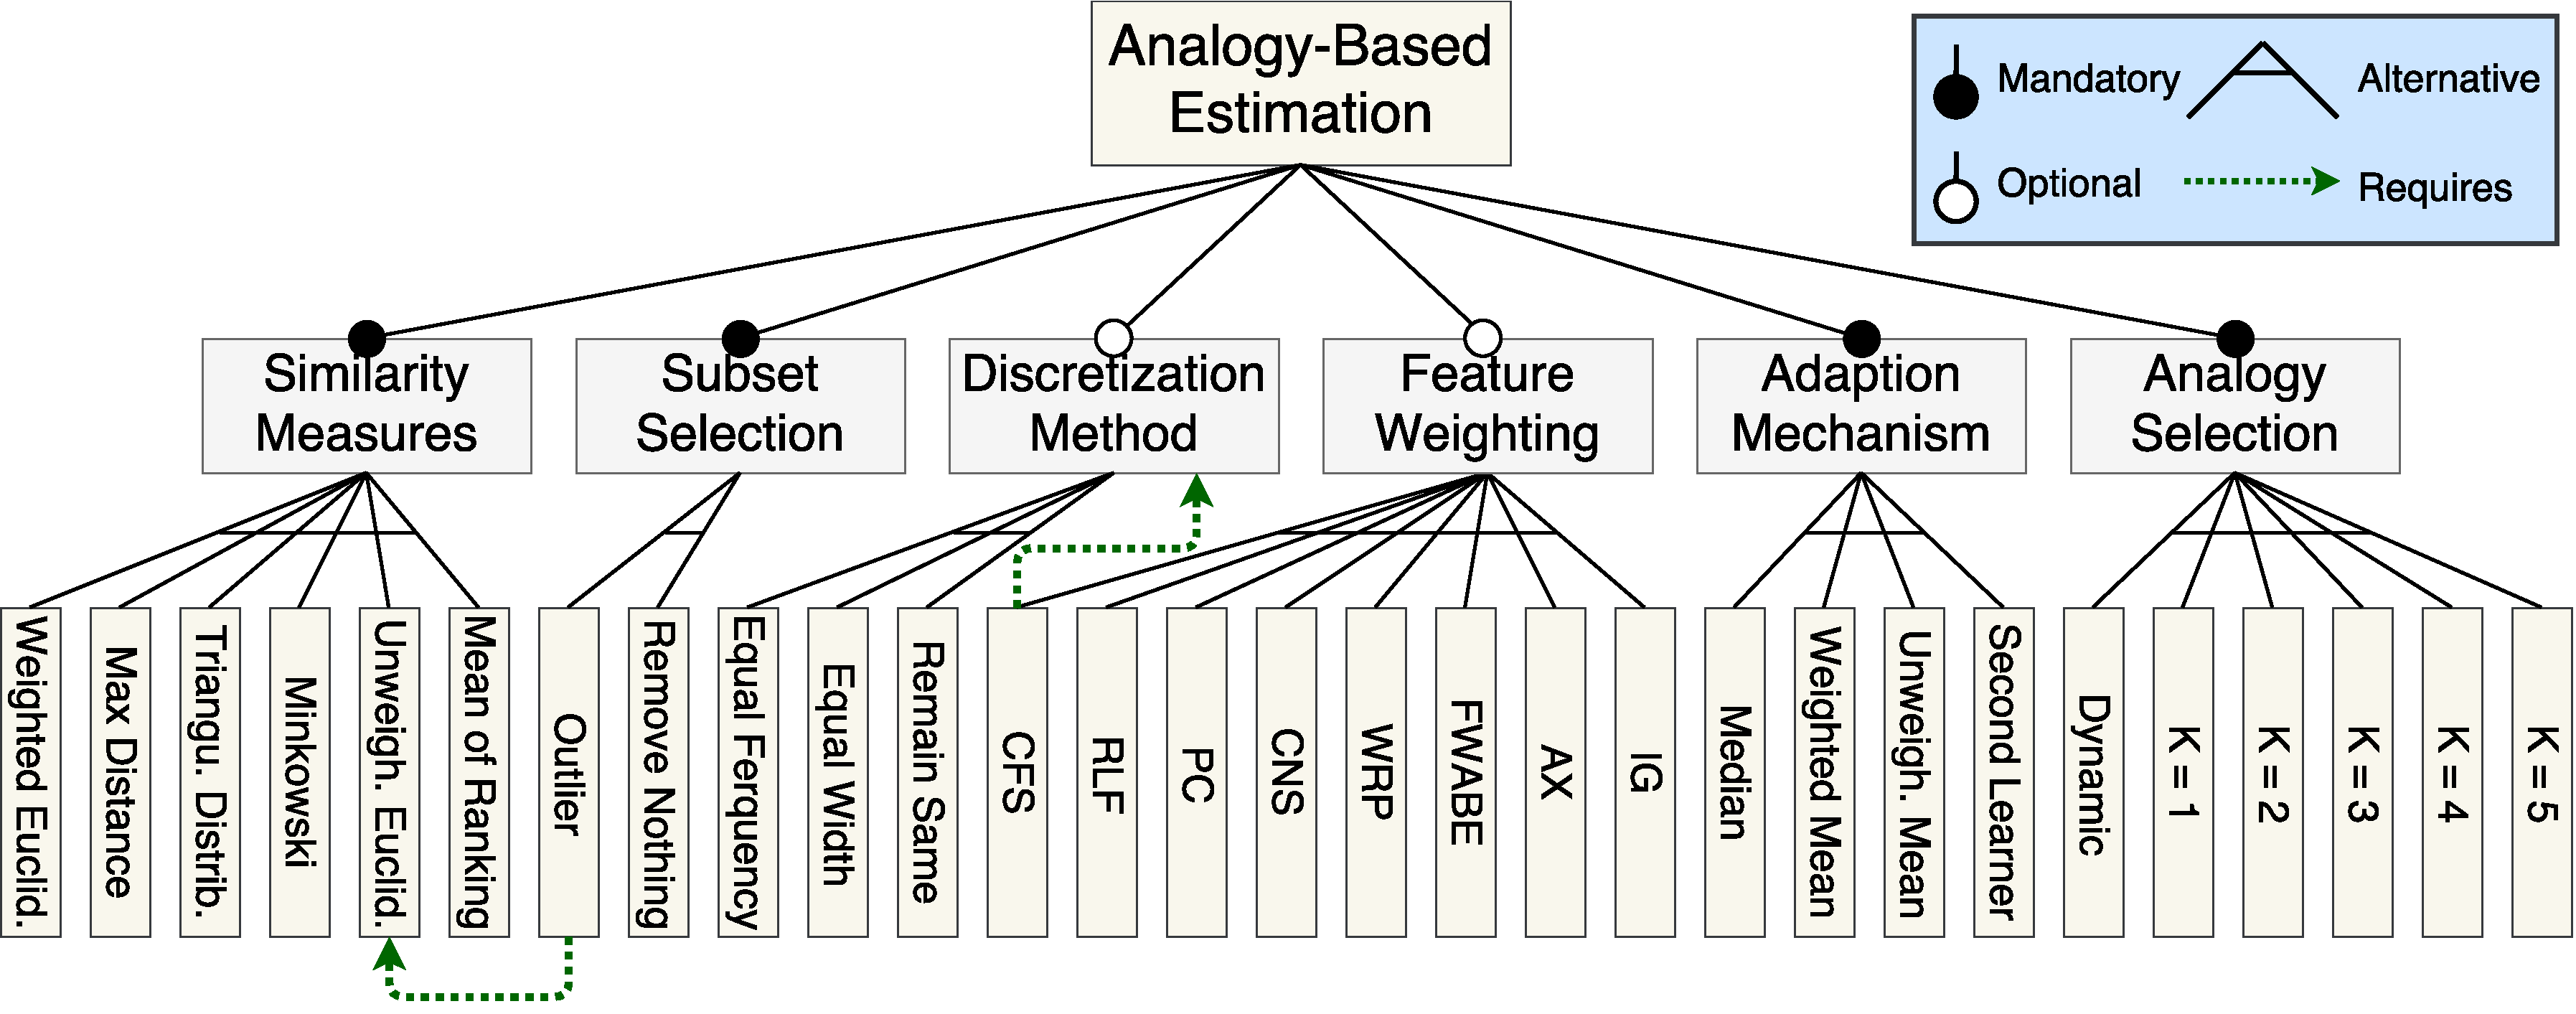
\includegraphics[width=.7\textwidth]{FTM.pdf}}
\caption{OIL's feature model of the space of machine learning options for ABEN.  In this model, $\mathit{Subset Selection}$, $\mathit{Similarity}$, $\mathit{Adaption Mechanism}$ and $\mathit{Analogy Selection}$ are the mandatory {\em features}, while the $\mathit{Feature Weighting}$ and $\mathit{Discretization Method}$ {\em features} are optimal. To avoid making the graph too complex, some cross-tree constrains are not presented.}    
\label{fig:featuretree}
\end{figure*}

\subsection{Effort Estimation and  Hyperparameter Optimization}
\label{sec:4}

Note that we do \underline{{\em not}} claim that the above represents all methods for  effort estimation. Rather, we  say that (a)~all the above are either prominent in the literature or widely used; and (b)~anyone  with knowledge of  the current effort estimation 
literature would be tempted to try some of the above.

While the above list is incomplete, it is certainly very long. Consider, for example, just the ABEN
variants documented in Table~\ref{tbl:aben}. There are 
$2\times 8\times 3\times 6\times 4\times 6=6,912$ such variants.  Some   can be ignored;
e.g. at $k=1$,     adaptation mechanisms return the same result, so they are not necessary. Also, not all  {\em feature} weighting techniques use discretization. But even after those discards, there are still thousands of possibilities. 

Given the space to exploration is so large, some researchers have offered automatic support for that exploration.
Some of that prior work suffered from being applied to limited data~\cite{li09} or optimizing
with algorithms that are not representative of  the state-of-the-art in multi-objective optimization~\cite{li09}.

Another issue with prior work is that researchers use methods  deprecated in the literature. 
For example,  some use grid search~\cite{dejaeger12,Song:2013}  which is a set of
nested for-loops that iterate over  a range of options.
Grid search is  slow and, due to the size of the increment in each loop, can miss important settings~\cite{Bergstra:2012}.

Other researchers assume that the effort model is a specific parametric form (e.g. the COCOMO equation)
and propose mutation methods to adjust the parameters of that equation~\cite{aljahdali2010software,Moeyersoms:2015,singh2012software,IJST70010,Rao14}. As mentioned above, this approach is
hard to test since there are very few data sets using the   pre-specified COCOMO attributes. 

Further, all that prior work needs to be revisited given the existence of recent and very prominent
methods; i.e. ATLM and CoGEE from TOSEM'15 and ICSE'16\cite{Whigham:2015,sarro2016multi}.


Accordingly, this paper conducts a  more thorough investigation of   hyperparameter optimization for effort estimation. 
\bi
\item
We  use methods with no   data
feature assumptions (i.e. no COCOMO data);
\item
That
 vary
many   parameters (6,000+ combinations);
\item
That also  tests  results   on 9 different sources with data on 945 software projects; 
\item
Which  uses optimizers   representative of the  state-of-the-art 
(NSGA-II~\cite{deb02}, MOEA/ D~\cite{Zhang07}, DE~\cite{storn1997differential});
\item
And which 
benchmark results 
against  prominent methods such as 
  ATLM and CoGEE.
\ei


\subsection{OIL}
\label{sec:5}


\pdfoutput=1
\begin{table*}[t!]
\caption{Descriptive Statistics of the Datasets}\label{table:dataset}
\renewcommand{\baselinestretch}{0.75} 
\centering
\begin{tabular}{cc}
\scriptsize
\begin{tabular}{|c|l|rrrr|}
    \hline
      & feature & min  & max & mean & std\\
   \hline

%%%%%%%%%%%%%%%%%%%%%%%%%%%%%%%%%%%%%%%%%%%%%%%%%%%%%%%%%%%%%%%%%%%%

\multirow{7}{*}{\begin{sideways}kemerer\end{sideways}}
& Langu. & 1 & 3 & 1.2 & 0.6\\
& Hdware & 1 & 6 & 2.3 & 1.7\\
& Duration & 5 & 31 & 14.3 & 7.5\\
& KSLOC & 39 & 450 & 186.6 & 136.8\\
& AdjFP & 100 & 2307 & 999.1 & 589.6\\
& RAWFP & 97 & 2284 & 993.9 & 597.4\\
& Effort & 23 & 1107 & 219.2 & 263.1\\
\hline
\multirow{8}{*}{\begin{sideways}albrecht\end{sideways}}
& Input & 7 & 193 & 40.2 & 36.9\\
& Output & 12 & 150 & 47.2 & 35.2\\
& Inquiry & 0 & 75 & 16.9 & 19.3\\
& File & 3 & 60 & 17.4 & 15.5\\
& FPAdj & 1 & 1 & 1.0 & 0.1\\
& RawFPs & 190 & 1902 & 638.5 & 452.7\\
& AdjFP & 199 & 1902 & 647.6 & 488.0\\
& Effort & 0 & 105 & 21.9 & 28.4\\
\hline
\multirow{12}{*}{\begin{sideways}isbsg10\end{sideways}}
% & Data\_Quality & 1 & 2 & 1.2 & 0.4\\
& UFP & 1 & 2 & 1.2 & 0.4\\
& IS & 1 & 10 & 3.2 & 3.0\\
& DP & 1 & 5 & 2.6 & 1.1\\
& LT & 1 & 3 & 1.6 & 0.8\\
& PPL & 1 & 14 & 5.1 & 4.1\\
& CA & 1 & 2 & 1.1 & 0.3\\
& FS & 44 & 1371 & 343.8 & 304.2\\
& RS & 1 & 4 & 1.7 & 0.9\\
% & Recording\_Method & 1 & 4 & 1.8 & 1.0\\
& FPS & 1 & 5 & 3.5 & 0.7\\
& Effort & 87 & 14453 & 2959 & 3518\\
\hline
\multirow{8}{*}{\begin{sideways}finnish\end{sideways}}
& hw & 1 & 3 & 1.3 & 0.6\\
& at & 1 & 5 & 2.2 & 1.5\\
& FP & 65 & 1814 & 763.6 & 510.8\\
& co & 2 & 10 & 6.3 & 2.7\\
& prod & 1 & 29 & 10.1 & 7.1\\
& lnsize & 4 & 8 & 6.4 & 0.8\\
& lneff & 6 & 10 & 8.4 & 1.2\\
& Effort & 460 & 26670 & 7678 & 7135\\
\hline

\end{tabular} 

%%%%%%%%%%%%%%%%%%%%%%%%%%%%%%%%%%%%%%%%%%%%%%%%%%%%%%%%%%%%%%%%%%%%


~

\scriptsize
\begin{tabular}{|c|l|rrrr|}
    \hline
      & feature
    & min  & max & mean & std\\
   \hline
%%%%%


\multirow{8}{*}{\begin{sideways}miyazaki\end{sideways}}
& KLOC & 7 & 390 & 63.4 & 71.9\\
& SCRN & 0 & 150 & 28.4 & 30.4\\
& FORM & 0 & 76 & 20.9 & 18.1\\
& FILE & 2 & 100 & 27.7 & 20.4\\
& ESCRN & 0 & 2113 & 473.0 & 514.3\\
& EFORM & 0 & 1566 & 447.1 & 389.6\\
& EFILE & 57 & 3800 & 936.6 & 709.4\\
& Effort & 6 & 340 & 55.6 & 60.1\\
\hline
\multirow{26}{*}{\begin{sideways}maxwell\end{sideways}}
& App & 1 & 5 & 2.4 & 1.0\\
& Har & 1 & 5 & 2.6 & 1.0\\
& Dba & 0 & 4 & 1.0 & 0.4\\
& Ifc & 1 & 2 & 1.9 & 0.2\\
& Source & 1 & 2 & 1.9 & 0.3\\
& Telon. & 0 & 1 & 0.2 & 0.4\\
& Nlan & 1 & 4 & 2.5 & 1.0\\
& T01 & 1 & 5 & 3.0 & 1.0\\
& T02 & 1 & 5 & 3.0 & 0.7\\
& T03 & 2 & 5 & 3.0 & 0.9\\
& T04 & 2 & 5 & 3.2 & 0.7\\
& T05 & 1 & 5 & 3.0 & 0.7\\
& T06 & 1 & 4 & 2.9 & 0.7\\
& T07 & 1 & 5 & 3.2 & 0.9\\
& T08 & 2 & 5 & 3.8 & 1.0\\
& T09 & 2 & 5 & 4.1 & 0.7\\
& T10 & 2 & 5 & 3.6 & 0.9\\
& T11 & 2 & 5 & 3.4 & 1.0\\
& T12 & 2 & 5 & 3.8 & 0.7\\
& T13 & 1 & 5 & 3.1 & 1.0\\
& T14 & 1 & 5 & 3.3 & 1.0\\
% & T15 & 1 & 5 & 3.3 & 0.7\\
& Dura. & 4 & 54 & 17.2 & 10.7\\
& Size & 48 & 3643 & 673.3 & 784.1\\
& Time & 1 & 9 & 5.6 & 2.1\\
& Effort & 583 & 63694 & 8223 & 10500\\
\hline

\end{tabular} 


%%%%%%%%%%%%%%%%%%%%%%%%%%%%%%%%%%%%%%%%%%%%%%%%%%%%%%%%%%%%%%%%%%%%

% ~

% \scriptsize
% \begin{tabular}{|c|l|rrrr|}
%     \hline
%       & feature
%     & min  & max & mean & std\\
%   \hline
% %%%%%


% \multirow{7}{*}{\begin{sideways}desharnais\end{sideways}}
% & TeamExp & 0 & 4 & 2.3 & 1.3\\
% & MngExp & 0 & 7 & 2.6 & 1.5\\
% & Length & 1 & 36 & 11.3 & 6.8\\
% & Trans.s & 9 & 886 & 177.5 & 146.1\\
% & Entities & 7 & 387 & 120.5 & 86.1\\
% & AdjPts & 73 & 1127 & 298.0 & 182.3\\
% & Effort & 546 & 23940 & 4834 & 4188\\
% \hline
% \multirow{7}{*}{\begin{sideways}kitchenham\end{sideways}}
% & code & 1 & 6 & 2.1 & 0.9\\
% & type & 0 & 6 & 2.4 & 0.9\\
% & duration & 37 & 946 & 206.4 & 134.1\\
% & fun\_pts & 15 & 18137 & 527.7 & 1522\\
% & estimate & 121 & 79870 & 2856 & 6789\\
% & esti\_mtd & 1 & 5 & 2.5 & 0.9\\
% & Effort & 219 & 113930 & 3113 & 9598\\
% \hline
% \multirow{19}{*}{\begin{sideways}china\end{sideways}}
% & ID & 1 & 499 & 250.0 & 144.2\\
% & AFP & 9 & 17518 & 486.9 & 1059\\
% & Input & 0 & 9404 & 167.1 & 486.3\\
% & Output & 0 & 2455 & 113.6 & 221.3\\
% & Enquiry & 0 & 952 & 61.6 & 105.4\\
% & File & 0 & 2955 & 91.2 & 210.3\\
% & Interface & 0 & 1572 & 24.2 & 85.0\\
% & Added & 0 & 13580 & 360.4 & 829.8\\
% & Changed & 0 & 5193 & 85.1 & 290.9\\
% & Deleted & 0 & 2657 & 12.4 & 124.2\\
% & PDR\_A & 0 & 84 & 11.8 & 12.1\\
% & PDR\_U & 0 & 97 & 12.1 & 12.8\\
% & NPDR\_A & 0 & 101 & 13.3 & 14.0\\
% & NPDU\_U & 0 & 108 & 13.6 & 14.8\\
% & Resource & 1 & 4 & 1.5 & 0.8\\
% & Dev.Type & 0 & 0 & 0.0 & 0.0\\
% & Duration & 1 & 84 & 8.7 & 7.3\\
% & N\_effort & 31 & 54620 & 4278 & 7071\\
% & Effort & 26 & 54620 & 3921 & 6481\\
% \hline

% \end{tabular}


%%%%%%%%%%%%%%%%%%%%%%%%%%%%%%%%%%%%%%%%%%%%%%%%%%%%%%%%%%%%%%%%%%%%


\end{tabular}
\end{table*}


  OIL is  our  architecture for exploring hyperparameter optimization and effort estimation,
  Initially, our plan
was to use standard hyperparameter  tuning for this task. Then we learned that standard data mining toolkits like scikit-learn~\cite{pedregosa2011scikit} did not include many of the effort estimation techniques; and (b) standard hyperparameter tuners can be  slow     (sklearn recommends a default runtime of 24 hours~\cite{sk18}).  Hence, we build OIL:
 \bi
 \item
At the base {\em library layer}, we use     Scikit-Learn~\cite{pedregosa2011scikit}. 
\item
Above that, OIL has a {\em utilities layer} containing all the algorithms missing in Scikit-Learn (e.g., ABEN required
numerous additions at the utilities layer). 
\item
Higher up, OIL's {\em modelling layer} uses an XML-based domain-specific language to specify a {\em feature} map of data mining options.
These feature models are single-parent and-or graphs with (optional) cross-tree constraints showing what options require or exclude other options.
A graphical representation of  the feature model used in this paper is shown in \fig{featuretree}.
\item
Finally, at top-most {\em optimizer layer}, there is some optimizer that  makes decisions across the {\em feature} map. An automatic {\em mapper} facility then links those decisions
down to the lower layers to run the selected algorithms.  
\ei

\subsection{Optimizers}
\label{sec:6}

\begin{wraptable}{r}{1.7in}
\vspace{-5pt}
\scriptsize
\caption{Data   in this study. For details on the features, see Table~\ref{table:dataset}.}\label{table:dataset_c}

~\\
\centering
\begin{tabular}{r|rr}
 	&Projects&	Features\\\hline
kemerer	&15&	6\\
albrecht&	24&	7\\
isbsg10&    37& 11\\
finnish	&38&	7\\
miyazaki&	48&	7\\
maxwell&	62	&25\\
desharnais&	77&	6\\
kitchenham& 145&    6\\
china&  499&    18\\\hline
total & 945
\end{tabular}
\vspace{-15pt}
\end{wraptable}

Once OIL's layers were  built, it was simple  to ``pop the top'' and replace the top
layer with another optimizer.
Nair et al.~\cite{nair18}   advise that for search-based SE studies, optimizers should be selecting
via the a 
  ``dumb+two+next''  rule. Here,   ``dumb'' is some baseline method;
``two'' are some  well-established optimizers;  and ``next'' is a more recent method which may not have been
applied before to this domain.

For our ``dumb''  optimizer, we used   Random Choice (hereafter, RD). To find $N$ valid configurations, RD
selects leaves at random from \fig{featuretree}.
All these $N$ variants are executed and the best one is selected for application to the test set. To maintain parity with   DE2 and DE8 systems described below, 
OIL uses  $N\in\{40,160\}$ (denoted RD40 and RD160). 

Moving on, our ``two'' well-established optimizer are differential evolution (hereafter, DE~\cite{storn1997differential}) and NSGA-II~\cite{deb02}. These have been used frequently in the SE literature\cite{Fu2016TuningFS,AGRAWAL2018,agrawal2017better,sayyad2013value,sayyad2013pareto}.
 NSGA-II is a standard genetic algorithm  (for N generations, mutate, crossover, select best candidates  for the next generation) with a fast   select operator. 
All candidates that dominated $i$ other items are grouped into together in ``band'' $i$.
When selecting $C$ candidates for the next generation, the top bands $1..i$ with $M< C$ candidates
are all selected.  Next, using a  near-linear time pruning operator, the $i+1$ band is pruned down to $C-M$ items, all of which are selected.


 The premise of DE is that the best way to mutate the existing tunings is to extrapolate between current solutions. Three solutions $a, b, c$ are selected at random. For each tuning parameter $k$, at some probability $cr$, we replace the old tuning $x_k$ with $y_k$. For
 booleans $y_k = \neg x_k$ and for numerics, 
\mbox{$y_k = a_k + f \times (b_k - c_k)$}
where $f$ is a
 parameter controlling cross-over.  
The main loop of DE runs over the population of size $np$, replacing old items with new candidates (if new candidate is better). This means that, as the loop progresses, the population is full of increasingly more valuable solutions (which, in turn,
helps   extrapolation). 
As to the control parameters of DE,  using advice from Storn~\cite{storn1997differential}, we set $\{\mathit{np,g,cr}\}=\{20,0.75,0.3\}$.
The number of generations $\mathit{gen}\in\{2,8\}$ was set as follows. A   small number (2) was used to test
the effects of  a very   CPU-light    effort estimator. A  larger number (8) was used to check if anything was
lost by restricting the inference to just two generations. These two versions were denoted DE2 and DE8.

As to our ``next'' optimizer, we used MOEA/D~\cite{Zhang07}.
This is a decomposition approach that
runs simultaneous   problems at once, as follows.  Prior to inference,
all candidates are assigned random weights to all  goals. Candidates
with similar weights are said to be in the same ``neighborhood''. When any candidate
 finds a useful mutation, then this candidate's
 values are copied to all neighbors that are further away than the candidate from the  best ``Utopian point''. Note that  these neighborhoods can be pre-computed and cached
prior to evolution. Hence, MOEA/D runs very quickly.
 MOEA/D has not been previously applied to effort estimation.

For these optimizers, DE and RD have the fixed evaluation budget  described above.
The other evolutionary treatments       (NSGA-II. MOEA/D, CoGEE)  were ran
till  the results from new generations were no better than before.

\section{Empirical Study} \label{sect:study} 

\subsection{Data}

\begin{table}
\caption{Performance scores: MRE and SA}\label{samre}
\begin{tabular}{|p{.95\linewidth}|}\hline
The performance   for our effort estimators are measured in terms of MRE and SA, defined in this table.
\\\hline
{\bf MRE:}
MRE is defined in terms of 
AR,  the magnitude of the absolute residual. This is  computed from the difference between predicted and actual effort values:
\[
\mathit{AR} = |\mathit{actual}_i - \mathit{predicted}_i|
\] 
MRE is the magnitude of the relative error calculated by expressing AR as a ratio of the actual effort value; i.e., 
\[
\mathit{MRE} = \frac{|\mathit{actual}_i - \mathit{predicted}_i|}{\mathit{actual}_i}
\]
MRE has been criticized~\cite{foss2003simulation,kitchenham2001accuracy,korte2008confidence,port2008comparative,shepperd2000building,stensrud2003further} as being biased towards error underestimations. 
\\\hline
{\bf SA:}
Because of issues with MRE, some researchers prefer the 
use of other (more standardized) measures, such as  Standardized Accuracy (SA)~\cite{langdon2016exact,shepperd2012evaluating}.
SA is defined in terms of 
\[
\mathit{MAE}=\frac{1}{N}\sum_{i=1}^n|\mathit{RE}_i-\mathit{EE}_i|
\]
where $N$ is the number of projects used for evaluating the performance, and $\mathit{RE}_i$ and $\mathit{EE}_i$ are the actual and estimated effort, respectively, for the project $i$. 
SA uses MAE as follows:
\[
\mathit{SA} = (1-\frac{\mathit{MAE}_{P_{j}}}{\mathit{MAE}_{r_{guess}}})\times 100
\]
where $\mathit{MAE}_{P_{j}}$ is the MAE of the approach $P_j$ being evaluated and $\mathit{MAE}_{r_{\mathit{guess}}}$ is the MAE of a large number (e.g., 1000 runs) of random guesses. 
Over many runs,  $\mathit{MAE}_{r_{\mathit{guess}}}$ will converge on simply using the sample mean~\cite{shepperd2012evaluating}. That is, SA represents how much better $P_j$ is than random guessing. Values near zero means that the prediction model $P_j$ is practically useless, performing little better than  random guesses~\cite{shepperd2012evaluating}. \\\hline
\end{tabular}
\end{table}

To assess OIL, we applied it to the 945 projects
seen in nine    datasets from the SEACRAFT repository (http://tiny.cc/seacraft); see Table~\ref{table:dataset} and Table~\ref{table:dataset_c}. 
This data was selected since it has been  widely  used in previous estimation research.
Also, it  is quite diverse since it differs for:
\bi
\item
Observation number (from 15 to 499 projects). 
\item
Number and type of {\em features} (from 6 to 25 {\em features}, including a variety of {\em features} describing the software projects, such as number of developers involved in the project and their experience, technologies used, size in terms of Function Points, etc.).
\item
Technical characteristics (software projects developed in different programming languages and for different application domains, ranging from telecommunications to commercial information systems).
\item
Geographical locations (software projects coming from Canada, China, Finland). 
\ei


\subsection{Cross-Validation}

Each data sets was treated in a variety of  ways. Each {\em treatment} is an {\em M*N-way} cross-validation test of some learner or some learner and optimizer. That is, $M$ times,  shuffle the data randomly (using a different random number seed)
then divide the data into $N$ bins.
For $i   \in N$, bin $i$ is used to test a model
build from the other bins.
Following the advice
of Nair et al.~\cite{nair18}, for the smaller data sets (with 40 rows or less), we  use $N=3$  bins
while for the others, we use $N=10$ bins.   

As a procedural detail, first we divided the data and then we applied the treatments. That is, all treatments saw the same training and test data.

\begin{figure}
\centering
{\scriptsize 
\begin{tabular}{llr@{~~~}r@{~~~}c} 
%\scriptsize
&  &\multicolumn{2}{c}{\textbf{MRE}} & \\ 
  {\textbf{Rank}}& \textbf{China} & \textbf{Med} & \textbf{IQR} & \\\hline 
   
   \rowcolor{gray!20}  1* &      CART\_DE8 &    8 &  1 & \quart{7}{1}{8}{100} \\
  \rowcolor{gray!20}   1* &      CART\_DE2 &    9 &  2 & \quart{8}{2}{9}{100} \\
    2 &      ABEN\_NSGA2 &    12 &  6 & \quart{12}{6}{12}{100} \\
    2 &      CART0 &    15 &  2 & \quart{14}{2}{15}{100} \\
    3 &      ABEN\_DE8 &    25 &  16 & \quart{18}{16}{25}{100} \\
    3 &      ABEN\_DE2 &    28 &  18 & \quart{20}{18}{28}{100} \\
    3 &      ABEN\_RD160 &    30 &  18 & \quart{23}{18}{30}{100} \\
    3 &      ABEN\_RD40 &    34 &  16 & \quart{26}{16}{34}{100} \\
    4 &      CART\_MOEAD &    40 &  10 & \quart{37}{10}{40}{100} \\
    4 &      CART\_NSGA2 &    40 &  17 & \quart{34}{17}{40}{100} \\
    5 &      ABE0 &    54 &  10 & \quart{47}{10}{54}{100} \\
    5 &      CoGEE &    57 &  11 & \quart{52}{11}{57}{100} \\
    6 &      ATLM &    69 &  18 & \quart{69}{18}{76}{100} \\
 \end{tabular}}
 
 \caption{Example of Scott-Knott results.
 MRE scores seen in  the China data set.
 sorted by their median value. 
 Here, {\em smaller} values are {\em better}.
  {\bf Med} is the 50th percentile and {\bf IQR} is the {\em inter-quartile range}; i.e., 75th-25th percentile. 
    Lines with a dot in the middle  shows   median values with the IQR.   
  For the  {\bf Ranks},  {\em smaller} values are  {\em better}.
   Ranks are computed via the Scott-Knot procedure from  TSE’15~\cite{Mittas13}.
    Rows with the same ranks
    are statistically indistinguishable. 
  \colorbox{gray!20}{1*} denotes rows of fastest best-ranked treatments.}\label{eg}
\end{figure}

\subsection{Scoring Metrics}

The results from each test set are evaluated in terms of two scoring metrics:  magnitude of the relative error (MRE)~\cite{Conte:1986:SEM:6176} and Standardized Accuracy (SA). These scoring metrics  are defined in Table~\ref{samre}.
We make no comment
on which   measure is better-- we use them since   they are widely used in the literature.

Note that for these evaluation measures:
\bi
\item {\em smaller} MRE values are {\em better};
\item
while {\em larger} SA values are {\em better}.
\ei
From this cross-validations,
we  report the {\em median} (sometimes shortened to {\em med})
which is the 50th percentile of the sorted test scores seen in the {\em M*N results}.
Also reported are the  {\em inter-quartile range} (sometimes shortened to {\em IQR}) which is the (75-25)th percentile.
The IQR is a  non-parametric
description of the   variability about the median value.  

For each data sets, the results from a {\em M*N-way} are sorted by their {\em  median} value, then {\em ranked} using the Scott-Knott test
recommended for ranking effort estimation experiments by Mittas et al. in TSE'15~\cite{Mittas13}. Scott-Knott is a top-down bi-clustering
method that recursively divides sorted treatments. Division stops when there is only one treatment left or when a division of numerous treatments generates 
splits that are statistically {\em indistinguishable}. 
To judge when two sets of treatments are indistinguishable, we use a conjunction of {\em both}  a 95\% bootstrap significance test~\cite{efron93} {\em and}
a A12 test for a non-small effect size difference in the distributions~\cite{MenziesNeg:2017}. These tests were used since their non-parametric nature avoids issues with non-Gaussian
distributions.  

Figure~\ref{eg} shows an example of the report generated by our Scott-Knott procedure.
Note that when multiple treatments tie for {\em Rank=1}, then we use the treatment's
runtimes to break the tie. Specifically, for all treatments in {\em Rank=1}, we mark the faster ones as \colorbox{gray!20}{{\em Rank=1*}}.

\subsection{Terminology for Optimizers}

Some treatments are named ``X\_Y'' which  denote learner ``X'' tuned by optimizer ``Y''.
In the following: 

{\small \begin{eqnarray} 
X &\in &\{\mathit{CART},\mathit{ABE}\}\nonumber\\
Y &\in &\{\mathit{DE2},\mathit{DE8},\mathit{MOEA/D},\mathit{NSGA2},\mathit{RD40}, \mathit{RD160}\}\nonumber
\end{eqnarray}}
Note that we do not tune CoGEE since, as shown in Table~\ref{tbl:runtime}, running that treatment even once is slow enough, let alone the hundred of re-runs required for additional tuning. Also, we do not tune ATLM since it was designed to be used ``off the shelf''.  Whigham et al.~\cite{Whigham:2015} declare that one of ATLM's most important features is that if does not need tuning.

\begin{figure*}
\renewcommand{\baselinestretch}{0.65} 
 \resizebox{0.45\textwidth}{!}{\begin{minipage}{4in}
{\small
\vspace{2.5mm}
\begin{center}a. \% MRE  ({\em smaller} values are {\em better}).\end{center}
\noindent \begin{tabular}{llrrc}
  {\textbf{Rank}}& \textbf{Using} & \textbf{Med.} & \textbf{IQR} & \\\hline
  
  \nm{china}\\
 \rowcolor{gray!20}   1* &      CART\_DE8 &    8 &  1 & \quart{7}{1}{8}{100} \\
 \rowcolor{gray!20}   1* &      CART\_DE2 &    9 &  2 & \quart{8}{2}{9}{100} \\ 
    2 &      CART0 &    15 &  2 & \quart{14}{2}{15}{100} \\
    4 &      CART\_MOEAD &    40 &  10 & \quart{37}{10}{40}{100} \\ 
    5 &      ABE0 &    54 &  10 & \quart{47}{10}{54}{100} \\ 
    6 &      ATLM &    69 &  18 & \quart{69}{18}{76}{100} \\\hline
  %%% generating from latex_plotting.py::plot_mre_for_all
\nm{albrecht}\\
    1 &      ABEN\_RD160 &    48 &  29 & \quart{36}{29}{48}{100} \\
    1 &      ABEN\_DE2 &    48 &  20 & \quart{40}{20}{48}{100} \\
 \rowcolor{gray!20}   1*&      ABE0 &    51 &  28 & \quart{39}{28}{51}{100} \\
    1 &      ABEN\_DE8 &    51 &  30 & \quart{36}{30}{51}{100} \\
 \rowcolor{gray!20}   1* &      CART\_DE8 &    52 &  28 & \quart{39}{28}{52}{100} \\
    2 &      CART\_DE2 &    56 &  23 & \quart{48}{23}{56}{100} \\
    2 &      CART\_MOEAD &    56 &  23 & \quart{48}{23}{56}{100} \\
    2 &      CART0 &    59 &  21 & \quart{48}{21}{59}{100} \\
    4 &      ATLM &    178 &  122 & \ofr \\\hline
\nm{desharnais}\\
    1 &      CoGEE &    35 &  14 & \quart{28}{14}{35}{100} \\
  \rowcolor{gray!20}   1* &      CART\_DE8 &    39 &  19 & \quart{31}{19}{39}{100} \\
  \rowcolor{gray!20}   1* &      CART\_DE2 &    41 &  19 & \quart{31}{19}{41}{100} \\
    2 &      CART\_MOEAD &    45 &  18 & \quart{37}{18}{46}{100} \\
    2 &      ATLM &    46 &  18 & \quart{37}{18}{46}{100} \\
    3 &      CART0 &    51 &  17 & \quart{46}{17}{51}{100} \\
    3 &      ABE0 &    56 &  33 & \quart{38}{33}{56}{100} \\
    \\
    \\
    \\
    \
\    \\
    \\
    \\
    \hline
\nm{finnish}\\
    \rowcolor{gray!20}   1* &      CART\_NSGA2 &    14 &  12 & \quart{8}{12}{14}{100} \\
    2 &      CART\_DE8 &    24 &  16 & \quart{16}{16}{24}{100} \\
    2 &      CART\_DE2 &    30 &  11 & \quart{24}{11}{30}{100} \\
    2 &      CART0 &    32 &  16 & \quart{25}{16}{32}{100} \\
    3 &      ABE0 &    43 &  26 & \quart{34}{26}{43}{100} \\
    4 &      CART\_MOEAD &    53 &  32 & \quart{49}{32}{53}{100} \\
    6 &      ATLM &    87 &  72 & \quart{49}{57}{87}{100} \\\hline
\nm{kemerer}\\
    \rowcolor{gray!20}   1* &      CART\_NSGA2 &    36 &  21 & \quart{31}{21}{33}{100} \\
    2 &      CART\_MOEAD &    46 &  15 & \quart{31}{15}{43}{100} \\
    2 &      CART\_DE2 &    54 &  22 & \quart{41}{22}{54}{100} \\
    2 &      ABE0 &    55 &  38 & \quart{32}{38}{55}{100} \\
    3 &      CART\_DE8 &    61 &  21 & \quart{49}{21}{61}{100} \\
    3 &      CART0 &    61 &  20 & \quart{52}{20}{61}{100} \\
    4 &      ATLM &    99 &  444 & \ofr \\
    \\
    \\
    \\
    \hline
\nm{maxwell}\\
  \rowcolor{gray!20}   1* &      CART\_DE8 &    43 &  26 & \quart{30}{26}{43}{100} \\
   \rowcolor{gray!20}   1* &      CART\_DE2 &    45 &  23 & \quart{33}{23}{45}{100} \\
    1 &      CoGEE &    45 &  17 & \quart{37}{17}{45}{100} \\
    2 &      ABE0 &    67 &  32 & \quart{51}{32}{67}{100} \\
    2 &      CART0 &    68 &  20 & \quart{56}{20}{68}{100} \\
    2 &      CART\_MOEAD &    75 &  28 & \quart{61}{28}{75}{100} \\
    3 &      ATLM &    540 &  917 & \ofr \\\hline
\nm{miyazaki}\\
  \rowcolor{gray!20}   1* &      CART\_DE8 &    42 &  27 & \quart{28}{27}{42}{100} \\
   \rowcolor{gray!20}   1* &      CART\_DE2 &    45 &  31 & \quart{31}{31}{45}{100} \\
    1 &      CART\_NSGA2 &    48 &  31 & \quart{31}{31}{48}{100} \\
    2 &      ABE0 &    56 &  35 & \quart{38}{35}{56}{100} \\
    2 &      CART0 &    56 &  20 & \quart{48}{20}{56}{100} \\
    3 &      CART\_MOEAD &    70 &  30 & \quart{65}{30}{70}{100} \\
    4 &      ATLM &    158 &  102 & \ofr \\\hline

\nm{isbsg10}\\
    1 &      CoGEE &    69 &  157 & \quart{57}{43}{69}{100} \\
  \rowcolor{gray!20}   1* &      CART\_DE2 &    72 &  15 & \quart{64}{15}{72}{100} \\
  \rowcolor{gray!20}   1*&      CART\_DE8 &    73 &  15 & \quart{64}{15}{73}{100} \\
  \rowcolor{gray!20}   1* &      ABE0 &    75 &  19 & \quart{64}{19}{75}{100} \\
 \rowcolor{gray!20}   1* &      CART0 &    75 &  10 & \quart{71}{10}{75}{100} \\
    2 &      CART\_MOEAD &    89 &  11 & \quart{83}{11}{89}{100} \\
    3 &      ATLM &    127 &  124 & \ofr \\
    \\
    \\
    \\
    \\
    \\
    \\
    \\
    \hline
\nm{kitchenham}\\
  \rowcolor{gray!20}   1* &      CoGEE &    12 &  7 & \quart{7}{7}{12}{100} \\
    2 &      ATLM &    26 &  12 & \quart{20}{12}{26}{100} \\
    2 &      CART\_DE2 &    26 &  10 & \quart{22}{10}{26}{100} \\
    2 &      CART\_DE8 &    27 &  11 & \quart{21}{11}{27}{100} \\
    2 &      CART0 &    34 &  11 & \quart{30}{11}{34}{100} \\
    4 &      ABE0 &    47 &  20 & \quart{36}{20}{47}{100} \\
    5 &      CART\_MOEAD &    69 &  32 & \quart{50}{32}{69}{100} \\
 %%% ----END HERE---------------------------------
  \end{tabular}} \end{minipage}}\hspace{12mm}
\resizebox{0.45\textwidth}{!}{\begin{minipage}{4in}
{\small
\begin{center}b. \% SA ({\em larger} values are {\em better})\end{center}

\noindent
\begin{tabular}{llrrc}
  {\textbf{Rank}}& \textbf{Using} & \textbf{Med.} & \textbf{IQR} & \\\hline 
\nm{china}\\
    \rowcolor{gray!20}   1*&      CART\_DE8 &    93 &  2 & \quart{92}{2}{93}{100} \\
 \rowcolor{gray!20}   1*&      CART\_DE2 &    93 &  2 & \quart{92}{2}{93}{100} \\
    3 &      CART0 &    85 &  7 & \quart{81}{7}{85}{100} \\
    4 &      ABE0 &    61 &  11 & \quart{56}{11}{61}{100} \\
    5 &      CART\_MOEAD &    54 &  19 & \quart{48}{19}{54}{100} \\
    5 &      ATLM &    48 &  7 & \quart{44}{7}{48}{100} \\\hline
    %%% generating from latex_plotting.py::plot_sa_for_all
\nm{albrecht}\\
 \rowcolor{gray!20}   1*&      CART\_MOEAD &    65 &  21 & \quart{60}{21}{65}{100} \\
    1 &      ABEN\_DE2 &    63 &  11 & \quart{56}{11}{63}{100} \\
    1 &      ABEN\_DE8 &    62 &  18 & \quart{50}{18}{62}{100} \\
    1 &      ABEN\_RD160 &    60 &  18 & \quart{50}{18}{60}{100} \\
   \rowcolor{gray!20}   1* &      ABE0 &    60 &  16 & \quart{52}{16}{60}{100} \\
    2 &      CART\_DE8 &    53 &  19 & \quart{42}{19}{53}{100} \\
    2 &      CART\_DE2 &    50 &  52 & \quart{10}{52}{50}{100} \\
    2 &      CART0 &    45 &  40 & \quart{20}{40}{45}{100} \\
    3 &      ATLM &    18 &  30 & \quart{13}{30}{18}{100} \\\hline

\nm{desharnais}\\
    1 &      CoGEE &    47 &  16 & \quart{40}{16}{47}{100} \\
    1 &      ABEN\_DE8 &    44 &  24 & \quart{28}{24}{44}{100} \\
    1 &      ABEN\_NSGA2 &    43 &  27 & \quart{27}{27}{43}{100} \\
   \rowcolor{gray!20}   1* &      ATLM &    42 &  13 & \quart{35}{13}{42}{100} \\
    1 &      ABEN\_RD40 &    42 &  27 & \quart{26}{27}{42}{100} \\
  \rowcolor{gray!20}   1* &      CART\_DE8 &    42 &  27 & \quart{26}{27}{42}{100} \\
    1 &      ABEN\_DE2 &    41 &  28 & \quart{24}{28}{41}{100} \\
   \rowcolor{gray!20}   1*&      CART\_DE2 &    40 &  26 & \quart{26}{26}{40}{100} \\
    1 &      ABEN\_RD160 &    40 &  31 & \quart{24}{31}{40}{100} \\
    2 &      CART\_MOEAD &    35 &  31 & \quart{15}{31}{35}{100} \\
    2 &      ABE0 &    30 &  42 & \quart{9}{42}{30}{100} \\
    2 &      CART0 &    23 &  18 & \quart{12}{18}{23}{100} \\\hline
\nm{finnish}\\    
   \rowcolor{gray!20}   1* &      CART\_DE8 &    81 &  14 & \quart{72}{14}{81}{100} \\
    2 &      CART\_DE2 &    74 &  10 & \quart{70}{10}{74}{100} \\
    2 &      CART\_MOEAD &    71 &  11 & \quart{70}{11}{71}{100} \\
    2 &      CART0 &    69 &  19 & \quart{55}{19}{69}{100} \\
    3 &      ABE0 &    49 &  22 & \quart{37}{22}{49}{100} \\
    4 &      ATLM &    40 &  49 & \quart{4}{49}{40}{100} \\
    \\
    \hline
\nm{kemerer}\\
   \rowcolor{gray!20}   1* &      CART\_MOEAD &    47 &  47 & \quart{23}{47}{47}{100} \\
    1 &      ABEN\_DE8 &    41 &  37 & \quart{24}{37}{41}{100} \\
    1 &      ABEN\_DE2 &    39 &  30 & \quart{26}{30}{39}{100} \\
   \rowcolor{gray!20}   1* &      ABE0 &    37 &  41 & \quart{20}{41}{37}{100} \\
    1 &      ABEN\_RD160 &    37 &  46 & \quart{10}{46}{37}{100} \\
    1 &      ABEN\_RD40 &    36 &  18 & \quart{28}{18}{36}{100} \\
    2 &      CART\_DE2 &    30 &  82 & \quart{-14}{63}{30}{100} \\
    2 &      CART\_DE8 &    26 &  102 & \quart{-14}{57}{26}{100} \\
    2 &      CART0 &    12 &  48 & \quart{-14}{48}{12}{100} \\
    3 &      ATLM &    -48 &  507 & \ofr \\\hline
\nm{maxwell}\\
   \rowcolor{gray!20}   1* &      CART\_MOEAD &    60 &  33 & \quart{44}{33}{60}{100} \\
    1 &      CoGEE &    59 &  20 & \quart{51}{20}{59}{100} \\
 \rowcolor{gray!20}   1* &      CART\_DE2 &    56 &  28 & \quart{38}{28}{56}{100} \\
    \rowcolor{gray!20}   1* &      CART\_DE8 &    56 &  31 & \quart{36}{31}{56}{100} \\
    2 &      ABE0 &    39 &  37 & \quart{18}{37}{39}{100} \\
    2 &      ATLM &    33 &  21 & \quart{28}{21}{33}{100} \\
    3 &      CART0 &    16 &  21 & \quart{2}{21}{16}{100} \\\hline
\nm{miyazaki}\\
   \rowcolor{gray!20}   1* &      CoGEE &    61 &  28 & \quart{43}{28}{61}{100} \\
    2 &      CART\_MOEAD &    51 &  31 & \quart{30}{31}{51}{100} \\
    2 &      CART\_DE8 &    45 &  36 & \quart{23}{36}{45}{100} \\
    3 &      CART\_DE2 &    41 &  36 & \quart{20}{36}{41}{100} \\
    3 &      ABE0 &    40 &  35 & \quart{21}{35}{40}{100} \\
    4 &      ATLM &    23 &  56 & \quart{-12}{56}{23}{100} \\
    \\[0.1cm]
    \hline

\nm{isbsg10}\\
  \rowcolor{gray!20}   1* &      CART\_MOEAD &    38 &  11 & \quart{29}{11}{38}{100} \\
    1 &      CART\_NSGA2 &    33 &  21 & \quart{15}{21}{33}{100} \\
    1 &      ABEN\_RD40 &    33 &  30 & \quart{15}{30}{33}{100} \\
    1 &      ABEN\_DE2 &    31 &  28 & \quart{16}{28}{31}{100} \\
    1 &      ABEN\_RD160 &    30 &  49 & \quart{-1}{49}{30}{100} \\
    1 &      ABEN\_DE8 &    28 &  57 & \quart{-4}{57}{28}{100} \\
   \rowcolor{gray!20}   1* &      ATLM &    28 &  19 & \quart{25}{19}{28}{100} \\
    \rowcolor{gray!20}   1* &      ABE0 &    28 &  29 & \quart{14}{29}{28}{100} \\
    1 &      ABEN\_NSGA2 &    26 &  33 & \quart{9}{33}{26}{100} \\
    1 &      CoGEE &    25 &  26 & \quart{12}{26}{25}{100} \\
    2 &      CART\_DE2 &    19 &  40 & \quart{-3}{40}{19}{100} \\
    2 &      CART\_DE8 &    16 &  20 & \quart{8}{20}{16}{100} \\
    2 &      CART0 &    15 &  24 & \quart{2}{24}{15}{100} \\\hline
\nm{kitchenham}\\
  \rowcolor{gray!20}   1* &      CoGEE &    90 &  6 & \quart{87}{6}{90}{100} \\
    2 &      ATLM &    79 &  8 & \quart{74}{8}{79}{100} \\
    2 &      CART\_DE2 &    77 &  12 & \quart{70}{12}{77}{100} \\
    2 &      CART\_DE8 &    76 &  12 & \quart{69}{12}{76}{100} \\
    3 &      ABE0 &    64 &  14 & \quart{56}{14}{64}{100} \\
    4 &      CART\_MOEAD &    58 &  22 & \quart{40}{22}{58}{100} \\
    4 &      CART0 &    56 &  15 & \quart{47}{15}{56}{100} \\


   %%% ----END HERE----------------------------------
   
   
  \end{tabular}
  }

\end{minipage}
}
 \caption{
\%  {\bf MRE} and \% {\bf SA} results
from our cross-validation studies. Same format as Figure~\ref{eg}.
The gray rows show the \colorbox{gray!20}{{\em Rank=1+} results} recommended
for each data set.
The phrase ``\ofr'' denotes results
that are so bad that they fall outside of the 0\%..100\% range shown here.
 For space reasons, these
results are slightly truncated.
Not shown here are  any {\em Rank$>1$} methods
that  are  listed as  {\em slower} in Table~\ref{tbl:runtime}
since   such sub-optimal and slower
 treatments need not be discussed further)
For
all results, see  tiny.cc/oil-18.
   }
 \label{fig:jur}
\end{figure*}




\section{Results}
 
\subsection{Observations}
 Figure~\ref{fig:jur} shows results from all
 data sets and both performance scores. 
 Table~\ref{tbl:runtime} shows the runtimes (in minutes) for all
 the techniques explored in this study.
 For space reasons,
 not 
 all treatments are shown in Figure~\ref{fig:jur}. Specifically, all the slower treatments
 (as defined in Table~\ref{tbl:runtime}) that were not ranked first   have been deleted (since such sub-optimal and slower
 treatments need not be discussed further). For a display of all the  results, see tiny.cc/oil-18.


In these results, we observe that ATLM performed as expected. Whigham etl.~\cite{Whigham:2015} designed this method to serve as a baseline against which other treatments can be compared. Hence, it might be
expected that   method will be defeated
by all others. This was certainly the
case here--
 as seen in Figure~\ref{fig:jur}, ATLM is not top-ranked in 16/18 of our results. 

Another thing to observe is that  random search (RD)  performed as expected; i.e. it was top-ranked in 0/18 results. This is a gratifying result since if random search was usually most effective, then that would negate the value of everything else studied in this paper.

CoGEE was observed to perform worse than expected. Sarro et al.~\cite{sarro2016multi} argued persuasively that CoGEE's
 multi-objective quest to reduce error and confidence interval was a better way to explore effort estimation. But while CoGEE was clearly the best method in the two kitchenham results of
 Figure~\ref{fig:jur}, the next ranked methods did not perform much worse (maximum performance loss is just 14\%). And those next-ranked methods were top-ranked in most of the other data sets. 
One issue we found with CoGEE was that there was no reference implementation 
available for the CoGEE   home page\footnote{www0.cs.ucl.ac.uk/staff/F.Sarro/projects/CoGEE}. Hence, we   built our own. This  
raises the possibility that our ``CoGEE'' is different to that reported at ICSE'16. For example, comparing their Table 1 of~\cite{sarro2016multi} to our Table~\ref{table:dataset}, 
they used fewer columns than us.
We conjecture that the CoGEE study included an undocumented feature selection component. 

Another losing treatment in these results was estimation-by-analogy. Prior to
this study, we viewed most of the effort estimation methods as somewhat equivalent.
But here we see that ABE achieves top-rank in only 5/18 of our data sets.  This implies that there is more useful structure in our  data than can be revealed
by merely asking a few nearest neighbors for the effort estimates.



\newcommand{\PP}{$< \! \! 1$}
\newcommand{\PM}{$< \! \! 30$}
\begin{table}[t!]
\caption{Mean runtime (in minutes), for one-way out of an N*M cross-validation
experiment. cross-validation (minutes). Executing on a 2GHz processor, 
with 8GB RAM,  running Windows 10. }\label{tbl:runtime}
\vspace{3mm}
\resizebox{1\textwidth}{!}{
\begin{tabular}{|r@{~}|r@{~}r@{~}r@{~}r@{~}r@{~}r@{~}|r@{~}r@{~}r@{~}r@{~}r@{~}r@{~}r|}\cline{2-14}
\multicolumn{1}{c|}{~}&\multicolumn{6}{c|}{fastest}&\multicolumn{7}{c|}{slower}\\\cline{2-14}
\multicolumn{1}{c|}{~}&	\begin{turn}{75}ABE0\end{turn}	&	\begin{turn}{75}CART0\end{turn}	&	\begin{turn}{75}ATLM\end{turn}&		\begin{turn}{75}CART\_DE2\end{turn}		&\begin{turn}{75}CART\_DE8\end{turn}	&	\begin{turn}{75}CART\_MOEAD\end{turn}	&	\begin{turn}{75}CART\_NSGA2\end{turn}	&	\begin{turn}{75}ABEN\_RD40\end{turn}	&	\begin{turn}{75}ABEN\_RD160\end{turn}	&	\begin{turn}{75}ABEN\_DE2\end{turn}	&	\begin{turn}{75}ABEN\_DE8\end{turn}	&	\begin{turn}{75}CoGEE\end{turn}	&	\begin{turn}{75}ABEN\_NSGA2\end{turn}\\\hline
kemerer	&  \PP	&\PP	&\PP	&\PP&	\PP&\PP&	5	&2&	5	&2	&4&	6&	17\\
albrecht&	\PP	&\PP	&\PP	&\PP&	\PP&\PP&	5&	2&	8	&3	&6&	7&	24\\
isbsg10&	\PP	&\PP	&\PP	&\PP&	\PP&\PP&	5&	4&	11	&4	&9&	15&	33\\
finnish&	\PP	&\PP	&\PP	&\PP&	\PP&\PP&	5&	3&	10	&4	&8&	9&	30\\
miyazaki&	\PP	&\PP	&\PP	&\PP&	\PP&\PP&	5&	4&	14	&5	&10	&12&	37\\
maxwell	&   \PP	&\PP	&\PP	&\PP&	\PP&\PP&	6&	13&	38	&16	&29&	37&	111\\
desharnais&	\PP	&\PP	&\PP	&\PP&	\PP&\PP&	4&	8&	19	&12	&22&	22&	64\\
kitchenham&	\PP	&\PP	&\PP	&\PP&	\PP&\PP&	6&	15&	32	&26& 48	&41	&126\\
china&   	\PP	&\PP	&\PP	&\PP&	\PP&\PP&	6&	36&	86	&82& 131& 133 &329\\\hline													
total	&3&	4&	4	&5&	5	&6	&47&	87&	223	&154	&267	&282	&771\\\hline
\end{tabular}
}
\end{table}


\subsection{Answers to Research Questions}

Finally, we turn to the research questions listed in the introduction.

 \noindent{\bf RQ1: Is is best just to use the ``off-the-shelf'' defaults?}
 
 As mentioned in the introduction, 
 Acuri \& Fraser note that for
 test case generation,   using the default settings
can work just as well as anything else. 
 We can see some evidence of this effect in  Figure~\ref{fig:jur}. Observe, for example, the
  kitcheham results where the untuned CoGEE treatment achieves {\em Rank=1*}.  
  
  That said,  Figure~\ref{fig:jur} is mostly negative on the use of default settings:
 \bi
 \item
In   12/18 of the results  of Figure~\ref{fig:jur}, there are
no   treatments that use the defaults found in  {\em Rank=1*}. 
 \item
 In 6  of the remainder, default
 treatments share {\em Rank=1*} status with some tuned learner. 
 \ei
 Another aspect to note in the Figure~\ref{fig:jur} results
 are the large differences in performance scores
 between the best and worst treatments (exceptions: albrecht and  isbsg10's MRE scores do not vary much). That is, there is much to be gained by using the {\em Rank=1+ treatments} and deprecating the rest.
 
 In summary,  using the defaults is recommended in very few
 data sets. Also, in terms of better test scores,
 there is much to be gained   from tuning. Hence. for effort estimation:
 
 \begin{result}{1}
``off-the-shelf'' defaults
 should be deprecated.
 \end{result}
 


 

\noindent{\bf RQ2: Can we replace the old   defaults
 with new defaults?}
 
 If the hyperparameter tunings found by this paper
 were nearly always the same, then this study
 could conclude by recommending better values
 for default settings. This would
 be a most convenient result since, 
 in future when new data arrives, the complexities of this study 
 would not be needed.
 
Unfortuneately, this turns out not to be the case.
Table~\ref{table:para_dist} shows the percent frequencies with which
some tuning decision appears in our {\em M*N-way} cross validations
(this table uses results from DE tuning CART since, as shown below,
this usually leads to best results).
If we count the times some tuning choice appears in more than 50\% of the datasets of that table, only one tuning decision seems moderately common:
\bi
\item
Use $\le 3$ min\_samples
in the leaves of a regression tree.
\ei
But even here, there are numerous examples
were that was not the best tuning.
Accordingly, we  say that Table~\ref{table:para_dist} shows that there is
much variations of the best tunings. 
Hence, for effort estimation:

 \begin{result}{2}
 Overall, there are no ``best'' default settings.
 \end{result}

Before going on, one curious aspect of the Table~\ref{table:para_dist} results are the 
\%max\_features results; it was rarely most useful to use all features. Except for our largest data set (china), best results were often obtained after discarding (at random) a quarter to three-quarters of the features. This is a clear indication that, in future work, it could be advantageous to explore more feature selection for CART models.

 
 

\noindent{\bf RQ3: Can we avoid slow hyperparameter optimization?}

``Kilo-optimizers'' such as  NSGA-II and CoGEE examine $10^3$ candidates or more
since  they explore population sizes
of $10^2$ for many generations. Hence, as shown in Table~\ref{tbl:runtime},
they can be very slow.

Is it possible to avoid such slow runtimes?
There are many heuristic methods for speeding up
kilo-optimization:
\bi
\item Active learners  select explore a few most informative candidates~\cite{krall15};
\item Decomposition learners like MOEA/D  convert large
objective problems into multiple smaller problems;
\item
Other optimizers   explore   fewer candidates (DE \& RD).
\ei

Kilo-optimization is necessary when their exploration of  more candidates leads to better solutions that heuristic exploration.
Such better solutions from kilo-optimization are rarely found in Figure~\ref{fig:jur} (only in 5/18 cases). Further, the size of the improvements
seen with kilo-optimizers   over the best Rank=2 treatments is very small (maximum performance drop=14\%).
Those improvements come at significant runtime cost (in Table~\ref{tbl:runtime}), the kilo-optimizers
are one to two orders of magnitude slower than other methods). Hence we say that for effort estimation:

\begin{result}{3}
Overall,  our  slowest  optimizers  perform  no
better than certain faster ones.
 \end{result}
 
\noindent{\bf RQ4: What  hyperparatmeter optimizers to use for effort estimation?}
To answer this question, we review
 three experimental procedures:
\be
\item
\underline{{\em ALL:}} Assuming no restrictions on total runtime or access to   CPU, a researcher
or industrial practitioner could run all the treatments reported in that paper
to generate their own version of Figure~\ref{fig:jur}. 
\item
\underline{{\em SOME:}} Alternatively, to avoid the methods deprecated in these results,
we could restrict the
processing  to just  CoGEE or  CART, where the latter is optimized by either DE8 or MOEA/D or NSGA-II.That combination generates best results in 18/18 of our results.
\item \underline{{\em MIN:}} 
Finally, a more pragmatic approach would be to run just CART, optimized by DE8 or MOEA/D. This approach achieves top-ranked results most of our results
(in 13/18 cases). 
\ee
Since there is no single best estimator, the  treatments suggested by 
\underline{{\em ALL}}, \underline{{\em SOME}}, \underline{{\em MIN}}
need to be assessed within a {\em M-N-way} cross-validation study.
If we follow the advice of Nair et al~\cite{nair18}, then
using the 25th to 75th percentile of the runtimes in   Table~\ref{tbl:runtime}, 
and assuming {\em M,N=3,10}, we predict:
\bi
\item
The \underline{{\em ALL}} procedure would take 37 to   164 hours to terminate (i.e. up to a week);
\item
The \underline{{\em SOME}} procedure would take 8.5 to 23 hours  (i.e. up to a day)
to  generate results
as good as ALL;
\item
Meanwhile the \underline{{\em MIN}}  procedure would take 1.5 hours to terminate to  generate the results
of  \underline{{\em SOME}}  (in 13/18 cases) and very nearly as good in the remaining 5 cases.
\ei
For pragmatic reasons we recommend \underline{{\em MIN}}.
Hence:
\begin{result}{4}
   For new data sets, try
CART
with the optimizers
MOEA/D
or
differential evolution
 \end{result}

\begin{table*}[!t]
\caption{Tunings discovered by hyperparameter selections
(CART+DE). Table rows
sorted by number of rows in data sets
(smallest on top).
Cells in this table show the percent of times a particular choice was made. White text on black denotes choices made in more than 50\% of tunings.
}\label{table:para_dist}
\begin{center}
%\renewcommand{\baselinestretch}{0.75} 
\footnotesize

\resizebox{1\linewidth}{!}{ 
\begin{tabular}{ r|c|c|c|c|c|c}

~ & \%max\_features & max\_depth & min\_sample\_split & min\_samples\_leaf  \\  
~ & (selected at random; & (of trees) & (continuation & (termination \\ 
~ & 100\% means ``use all'') &   & criteria) & criteria)   \\\cline{2-7} 
~ &
\makecell[l]{
\ 25\%\ 50\%\ 75\%\ 100\%} &
\makecell[l]{
\ $\leq$03 \ $\leq$06 \ $\leq$09 \ $\leq$12} &
\makecell[l]{
\ $\leq$5 \ $\leq$10 \ $\leq$15 \ $\leq$20} &
\makecell[l]{
\ $\leq$03 \ $\leq$06 \ $\leq$09 \ $\leq$12} 
 \\
\hline


% kemerer 
% &\dbox{28}\dbox{22}\dbox{28}\dbox{22} 
% &\wbox{99}\dbox{00}\dbox{00}\dbox{00} 
% &\wbox{68}\dbox{15}\dbox{10}\dbox{07} 
% &\wbox{73}\dbox{08}\dbox{12}\dbox{07}\\ 

% albrecht 
% &\dbox{20}\dbox{28}\dbox{25}\dbox{27} 
% &\wbox{99}\dbox{00}\dbox{00}\dbox{00} 
% &\wbox{55}\dbox{43}\dbox{02}\dbox{00} 
% &\wbox{98}\dbox{00}\dbox{02}\dbox{00}\\ 

% isbsg10 
% &\dbox{20}\dbox{32}\dbox{28}\dbox{20} 
% &\wbox{99}\dbox{00}\dbox{00}\dbox{00} 
% &\dbox{45}\dbox{25}\dbox{22}\dbox{08}
% &\wbox{78}\dbox{18}\dbox{02}\dbox{02}\\ 

% finnish 
% &\dbox{07}\dbox{10}\dbox{35}\dbox{48} 
% &\wbox{99}\dbox{00}\dbox{00}\dbox{00} 
% &\wbox{55}\dbox{32}\dbox{05}\dbox{08} 
% &\wbox{83}\dbox{17}\dbox{00}\dbox{00}\\ 

% miyazaki 
% &\dbox{09}\dbox{23}\dbox{33}\dbox{35} 
% &\wbox{98}\dbox{02}\dbox{00}\dbox{00} 
% &\dbox{40}\dbox{27}\dbox{18}\dbox{15} 
% &\wbox{69}\dbox{23}\dbox{05}\dbox{03}\\ 

% maxwell 
% &\dbox{09}\dbox{14}\dbox{39}\dbox{38} 
% &\wbox{99}\dbox{00}\dbox{00}\dbox{00} 
% &\dbox{41}\dbox{32}\dbox{17}\dbox{10} 
% &\wbox{63}\dbox{33}\dbox{03}\dbox{01}\\ 

% desharnais
% &\dbox{17}\dbox{21}\dbox{40}\dbox{22} 
% &\wbox{98}\dbox{02}\dbox{00}\dbox{00} 
% &\dbox{32}\dbox{29}\dbox{18}\dbox{21} 
% &\dbox{40}\dbox{38}\dbox{19}\dbox{03}\\ 

% kitchenham
% &\dbox{02}\dbox{17}\dbox{33}\dbox{48} 
% &\wbox{95}\dbox{05}\dbox{00}\dbox{00} 
% &\dbox{32}\dbox{28}\dbox{21}\dbox{19} 
% &\wbox{56}\dbox{28}\dbox{09}\dbox{07}\\ 

% china 
% &\dbox{00}\dbox{07}\dbox{37}\wbox{56} 
% &\wbox{51}\dbox{49}\dbox{00}\dbox{00} 
% &\dbox{49}\dbox{32}\dbox{14}\dbox{05} 
% &\wbox{79}\dbox{20}\dbox{01}\dbox{00}\\ 

kemerer
&\dbox{18}\dbox{32}\dbox{23}\dbox{27}
&\wbox{57}\dbox{37}\dbox{05}\dbox{00}
&\wbox{95}\dbox{02}\dbox{03}\dbox{00}
&\wbox{92}\dbox{02}\dbox{05}\dbox{02}
\\
albrecht
&\dbox{13}\dbox{23}\dbox{20}\dbox{43}
&\wbox{63}\dbox{28}\dbox{08}\dbox{00}
&\wbox{68}\dbox{32}\dbox{00}\dbox{00}
&\wbox{83}\dbox{15}\dbox{02}\dbox{00}
\\
isbsg10
&\dbox{12}\dbox{35}\dbox{28}\dbox{25}
&\wbox{57}\dbox{33}\dbox{08}\dbox{00}
&\dbox{47}\dbox{23}\dbox{15}\dbox{15}
&\wbox{60}\dbox{27}\dbox{10}\dbox{03}
\\
finnish
&\dbox{07}\dbox{03}\dbox{27}\wbox{63}
&\dbox{32}\wbox{56}\dbox{12}\dbox{00}
&\wbox{73}\dbox{18}\dbox{05}\dbox{03}
&\wbox{78}\dbox{17}\dbox{05}\dbox{00}
\\
miyazaki
&\dbox{10}\dbox{22}\dbox{27}\dbox{40}
&\dbox{31}\dbox{46}\dbox{20}\dbox{03}
&\dbox{42}\dbox{24}\dbox{18}\dbox{16}
&\wbox{78}\dbox{13}\dbox{07}\dbox{02}
\\
maxwell
&\dbox{04}\dbox{16}\dbox{40}\dbox{40}
&\dbox{18}\wbox{60}\dbox{20}\dbox{02}
&\dbox{44}\dbox{27}\dbox{17}\dbox{12}
&\wbox{50}\dbox{33}\dbox{14}\dbox{04}
\\
desharnais
&\dbox{25}\dbox{23}\dbox{27}\dbox{25}
&\dbox{40}\dbox{46}\dbox{11}\dbox{02}
&\dbox{36}\dbox{26}\dbox{13}\dbox{25}
&\dbox{32}\dbox{26}\dbox{24}\dbox{19}
\\
kitchenham
&\dbox{01}\dbox{12}\dbox{32}\wbox{56}
&\dbox{03}\dbox{42}\dbox{45}\dbox{10}
&\dbox{43}\dbox{30}\dbox{17}\dbox{10}
&\dbox{48}\dbox{35}\dbox{12}\dbox{04}
\\
china
&\dbox{00}\dbox{04}\dbox{25}\wbox{71}
&\dbox{00}\dbox{00}\dbox{25}\wbox{75}
&\wbox{56}\dbox{30}\dbox{10}\dbox{02}
&\wbox{68}\dbox{28}\dbox{04}\dbox{00}
\\\end{tabular}}

\mbox{KEY: \colorbox{black!10}{\bf 10}\colorbox{black!20}{\bf 20}\colorbox{black!30}{\bf 30}\colorbox{black!40}{\bf 40}\colorbox{black!50}{\bf \textcolor{white}{50}}\colorbox{black!60}{\bf \textcolor{white}{60}}\colorbox{black!70}{\bf \textcolor{white}{70}}\colorbox{black!80}{\bf \textcolor{white}{80}}\colorbox{black!90}{\bf \textcolor{white}{90}}\colorbox{black}{\bf \textcolor{white}{100}}}\%


\end{center}
\end{table*}

\section{Threats to Validity}\label{sect:threats}
 \textbf{Internal Bias:} Many of  our methods contain stochastic random operators. To reduce the bias from random operators, we 
repeated our experiment in 20 times and applied statistical tests to remove spurious distinctions.

 \textbf{Parameter Bias:} For other studies, this is a significant question
 since (as shown above) the settings to the control parameters of the learners
 can have a dramatic effect on the efficacy of the estimation.
 That said, 
 recall that much of the technology of this paper concerned methods to explore
 the space of possible parameters.
 Hence we assert that 
 this study suffers much less paramter bias than other studies.
 
%  DE plays an important role in OIL, in this paper, we did not discuss the influence of different DE
% parameters, such as $cr$, $np$, $f$. In this paper, we followed Storn {\it et al.}'s configurations~\cite{storn1997differential}. Clearly, tuning such parameters is
% a direction for  future work.


\textbf{Sampling Bias:} While we tested OIL on the nine datasets, it would be inappropriate to conclude that OIL tuning  always perform better than
others methods for all data sets.
As researchers, what we can do to mitigate this problem is to carefully document out method, release out code,
and encourage the community to try this method on more datasets, as the occasion arises.


\section{Conclusions and Futurte Work} \label{sect:conclusion}

Hyperparameter optimization is known to dramatically improve the performance of many software analytics tasks such as software defect prediction or 
 text classification \cite{Fu2016TuningFS,tanti18,AGRAWAL2018,agrawal2017better}.
But as discussed in   \S\ref{sec:4}, the  benefits of      hyperparameter  optimization for   effort estimation 
have not been extensively
studied.
Prior work in this area only explored very small data sets~\cite{li09} or used
optimization
  algorithms that are not representative of  the state-of-the-art in multi-objective optimization~\cite{li09,dejaeger12,Song:2013}.
Other researchers assume that the effort model is a specific parametric form (e.g. the COCOMO equation), which greatly limits the amount of data that can be studied.
Further, all that prior work needs to be revisited given the existence of recent and very prominent
methods; i.e. ATLM and CoGEE from TOSEM'15 and ICSE'16\cite{Whigham:2015,sarro2016multi}.

Accordingly, this paper conducts a  more thorough investigation of     hyperparameter   optimization for effort estimation
using methods (a)~with no   data
feature assumptions (i.e. no COCOMO data);
(b)~that
 vary
many  parameters (6,000+ combinations);
that    tests  its results   on 9 different sources with data on 945 software projects; 
(c)~which  uses optimizers   representative of the  state-of-the-art 
(NSGA-II~\cite{deb02}, MOEA/D~\cite{Zhang07}, DE~\cite{storn1997differential});
and which 
(d)~benchmark results 
against  prominent methods such as 
  ATLM and CoGEE.

These results were assessed with respect to the  Acuri and  Fraser's concerns mentioned in the introduction; i.e. sometimes
hyperparamter optimization can be both too slow and not effective.
Such pessimism    may indeed apply  to  the  test  data  generation  domain.
However, 
the results of this paper show that 
 there  exists
other domains like effort estimation where hyperparameter
optimization  is  both
useful
and
fast. After  applying  hyperparamter optimization,  large  improvements  in  effort
estimation  accuracy  were  observed  (measured  in  terms  of  the
magnitude  of  the  relative  error  and  standardized  accuracy).
From those results, we can recommend using regression trees
(CART)  tuned  by  either  different  evolution  or  MOEA/D.  This
particular combination of learner and optimizers can achieve
in  one  or  two  hours  what  other  optimizers  need  days  to  weeks
of  CPU  to  accomplish.

To the best of our knowledge,
this study is the most extensive exploration   of
hyperparameter optimization and effort estimation yet undertaken. That said, there are very many
options not explored here. Our current
plans for future work include the following.
\bi
\item Try other learners:
e.g. neural nets, bayesian learners;
\item Try other data pre-processors.
We mentioned above how it was curious that
max features was often less than 100\%.
This is a clear indication that, we
might be able to further improve our estimations results by adding
more intelligent feature selection to, say, CART.
\item Other optimizers. For example,
combining DE and MOEA/D might be a fruitful way
to proceed.
\item Yet another possible future direction
could be hyper-hyperparamter optimization. In
the above, we used optimizers like differential
evolution to tune learners. But these optimizers
have their own control parameters. Perhaps there 
are better settings for the optimizers? Which could be found via hyper-hyperparameter optimization?
\ei
Hyper-hyperparameter optimization could be a very slow
process. Hence, results like this paper could be
most useful since here we have identified
optimizers that are
very fast and very slow (and the latter would
not be suitable for hyper-hyperparamter optimization).

In any case,
we  hope  that
OIL  and the results of this paper will  prompt  and  enable
much more research on better methods to tune software effort
estimators
To that end, we have placed all our scripts and data   on-line at http://blinded4review.

\section*{Acknowledgement}
Funding source grant number blinded for review.


% \begin{acknowledgements}
% Funding source grant number blinded for review.
% \end{acknowledgements}

% BibTeX users please use one of
%\bibliographystyle{spbasic}      % basic style, author-year citations
%\bibliographystyle{spmpsci}      % mathematics and physical sciences
%\bibliographystyle{spphys}       % APS-like style for physics
%\bibliography{}   % name your BibTeX data base

% Non-BibTeX users please use
% \begin{thebibliography}{}
%
% and use \bibitem to create references. Consult the Instructions
% for authors for reference list style.
%

% \bibitem{RefJ}
% % Format for Journal Reference
% Author, Article title, Journal, Volume, page numbers (year)
% % Format for books
% \bibitem{RefB}
% Author, Book title, page numbers. Publisher, place (year)
% % etc

% \bibliographystyle{spmpsci}
\bibliographystyle{IEEEtran}
% \bibliography{sigproc} 
\bibliography{reference}


% \end{thebibliography}

\end{document}

